%%%%%%%%%%%%%%%%%%%%%%%%%%%%%%%%%%%%%%%%%%%%%%%%%%%%%%%%%%%%%%%%%%%%%%%%%%%%
%%%%%                          ANNEXE 2                               %%%%%%
%%%%%%%%%%%%%%%%%%%%%%%%%%%%%%%%%%%%%%%%%%%%%%%%%%%%%%%%%%%%%%%%%%%%%%%%%%%%

%\renewcommand{\thesection}{\Alph{section}}
%\setcounter{section}{2}
\phantomsection 

\lhead[\fancyplain{}{\leftmark}]%Pour les pages paires \bfseries
      {\fancyplain{}{}} %Pour les pages impaires
\chead[\fancyplain{}{}]%
      {\fancyplain{}{}}
\rhead[\fancyplain{}{}]%Pour les pages paires 
      {\fancyplain{}{\rightmark}}%Pour les pages impaires \bfseries
\lfoot[\fancyplain{}{}]%
      {\fancyplain{}{}}
\cfoot[\fancyplain{}{\thepage}]%\bfseries
      {\fancyplain{}{\thepage}} %\bfseries
\rfoot[\fancyplain{}{}]%
     {\fancyplain{}{\scriptsize}}


%%%%%%%%%%%%%%%%%%%%%%%%%%%%%%%%%%%%%%%%%%%%%%%%%%%%%%%%%%%%%%%%%%%%%%%%%%
%%%%%                      Start part here                          %%%%%%
%%%%%%%%%%%%%%%%%%%%%%%%%%%%%%%%%%%%%%%%%%%%%%%%%%%%%%%%%%%%%%%%%%%%%%%%%%

\chapter{Impact de la gaine rigide sur la relation entre le bras de levier de VH et la hauteur de flambement}
\label{Ann:2_calcul a_la avec Dg, x0 et Dte fixes}

\minitoc
\newpage

%%/!\/!\/!\/!\/!\/!\/!\/!\/!\/!\/!\/!\/!\/!\/!\/!\/!\/!\/!\/!\/!\/!\/!\/!\
%\section{Cinématique de pliage de la VH avant saut}
%\label{sec:A1.1_Cinématique de pliage de la VH avant saut}
%%/!\/!\/!\/!\/!\/!\/!\/!\/!\/!\/!\/!\/!\/!\/!\/!\/!\/!\/!\/!\/!\/!\/!\/!\
%
%%%%%%%%%%%%%%%%%%%%%%%%%%%%%%%%%%%%%	
%\begin{figure}[!htb]
%\begin{center}
%    \captionsetup{justification=centering} 
%	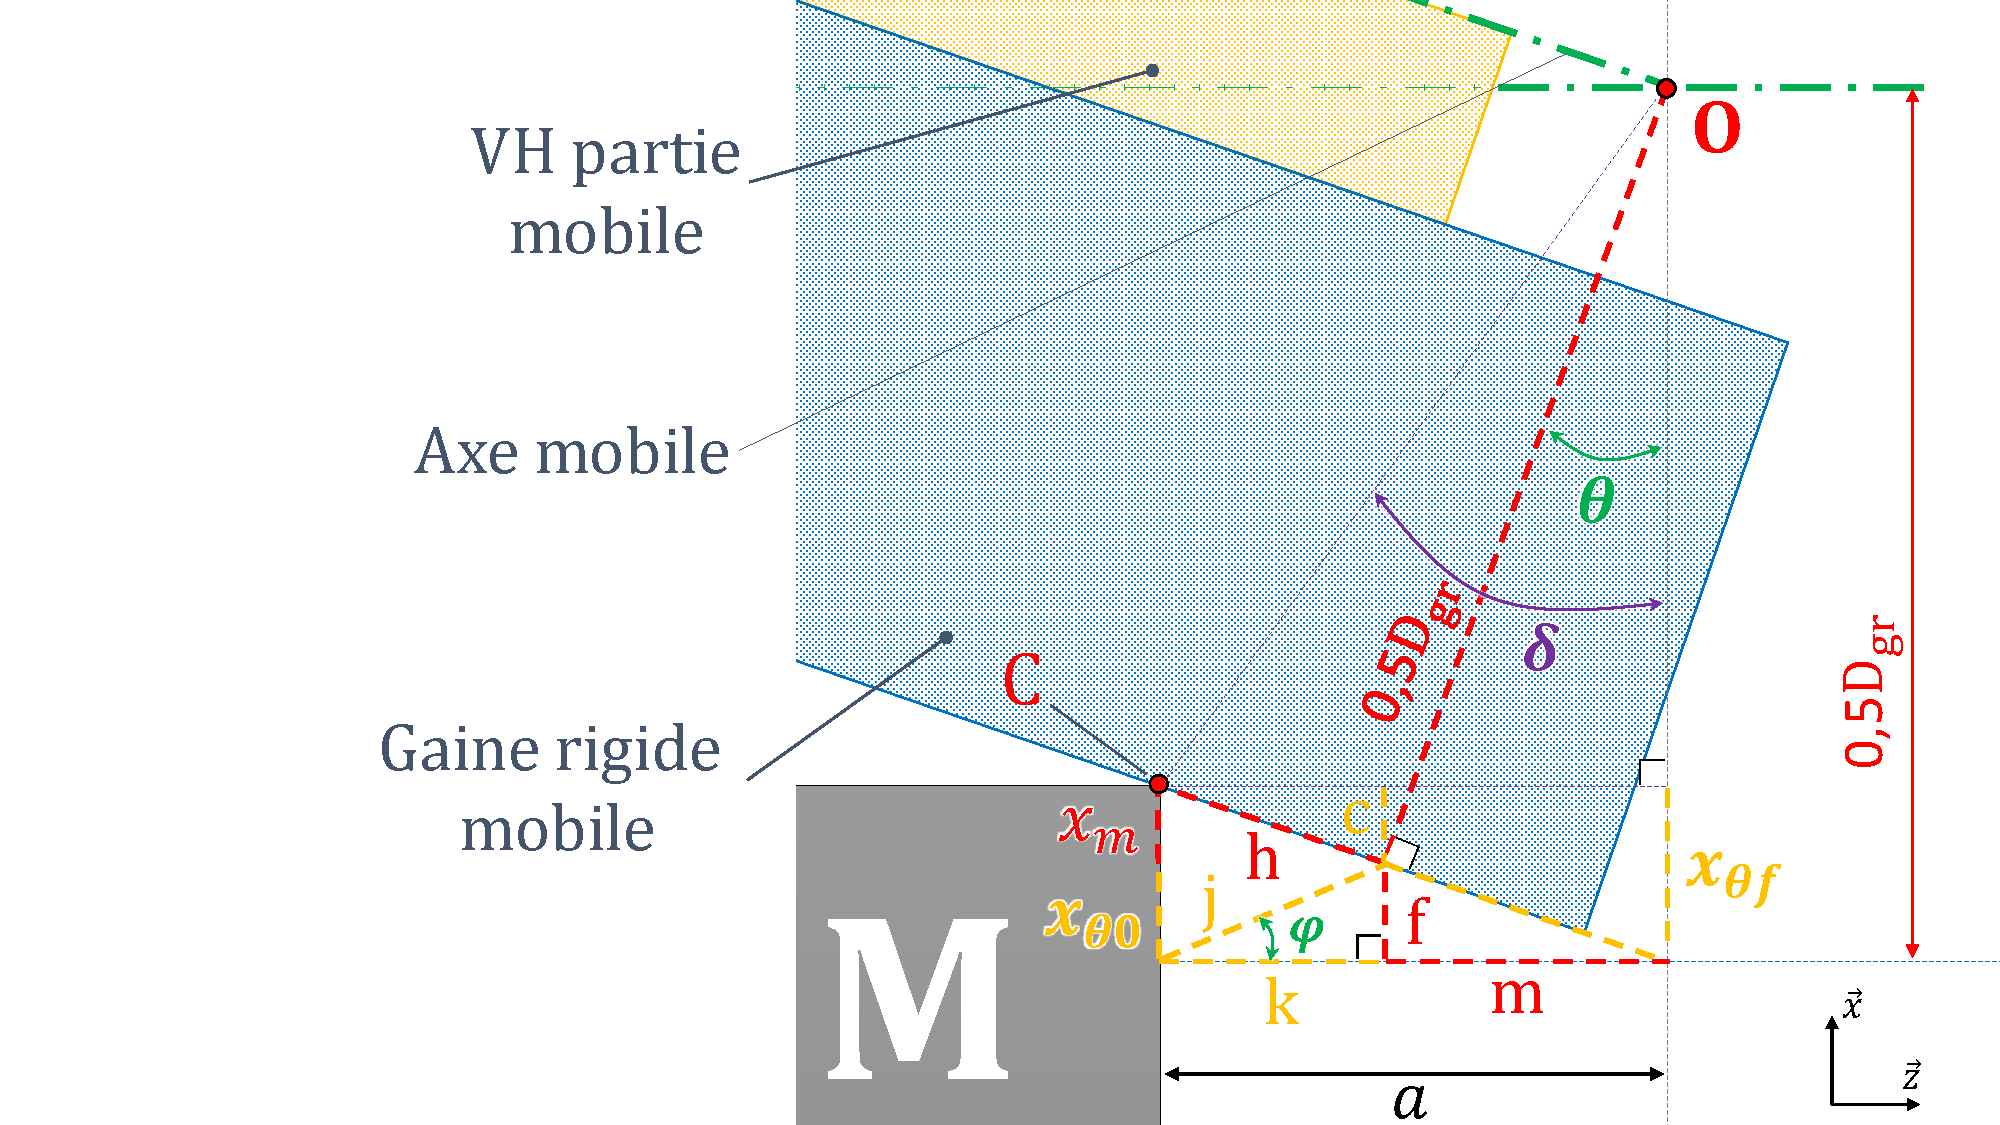
\includegraphics[trim={6cm 0cm 0cm 0cm},clip, 					                 width=\textwidth]{../Chap6/Figure/cinematique_pliage_VH_lacher_calculs.pdf}
%	\caption{Schéma de la configuration de pliage de la VH tenant compte de la gaine rigide avant le saut}
%	\label{fig:presentation_BDT}
%\end{center}	
%\end{figure}  
%\FloatBarrier     
%%%%%%%%%%%%%%%%%%%%%%%%%%%%%%%%%%%%%
%
%
%
%\begin{subnumcases}{}
%$$
%f_0 = \dfrac{D_g}{2}\ (1-\cos(\theta_0))
%$$
%\label{eq:An2_f0}\\
%$$
%m_0 = \dfrac{D_g}{2}\ sin(\theta_0)
%$$
%\label{eq:An2_m0}\\
%$$
%k_0 = a_0 - m_0
%$$
%\label{eq:An2_k0}\\
%$$
%\varphi_0 = \arctan\biggl(\dfrac{f_0}{k_0}\biggr)
%$$
%\label{eq:An2_varphi0}\\
%$$
%j_0 = \dfrac{k_0}{\cos(\varphi_0)}
%$$
%\label{eq:An2_j0}\\
%$$
%h_0 = \dfrac{k_0}{\cos(\theta_0)}
%$$
%\label{eq:An2_h0}\\
%$$
%c_0 = h_0 \sin(\theta_0)
%$$
%\label{eq:An2_c0}\\
%$$
%\delta_0 = \arctan\Biggl(\dfrac{2\ h_0}{D_g}\Biggr)
%$$
%\label{eq:An2_del0}\\
%$$
%x_{t0} = c_0 + f_0
%$$
%\label{eq:An2_xt0}\\
%\end{subnumcases} 
%
%
%%/!\/!\/!\/!\/!\/!\/!\/!\/!\/!\/!\/!\/!\/!\/!\/!\/!\/!\/!\/!\/!\/!\/!\/!\
%\section{Cinématique de pliage de la VH après saut}
%\label{sec:A1.1_Cinématique de pliage de la VH après saut}
%%/!\/!\/!\/!\/!\/!\/!\/!\/!\/!\/!\/!\/!\/!\/!\/!\/!\/!\/!\/!\/!\/!\/!\/!\
%
%%%%%%%%%%%%%%%%%%%%%%%%%%%%%%%%%%%%%	
%\begin{figure}[!htb]
%\begin{center}
%    \captionsetup{justification=centering} 
%	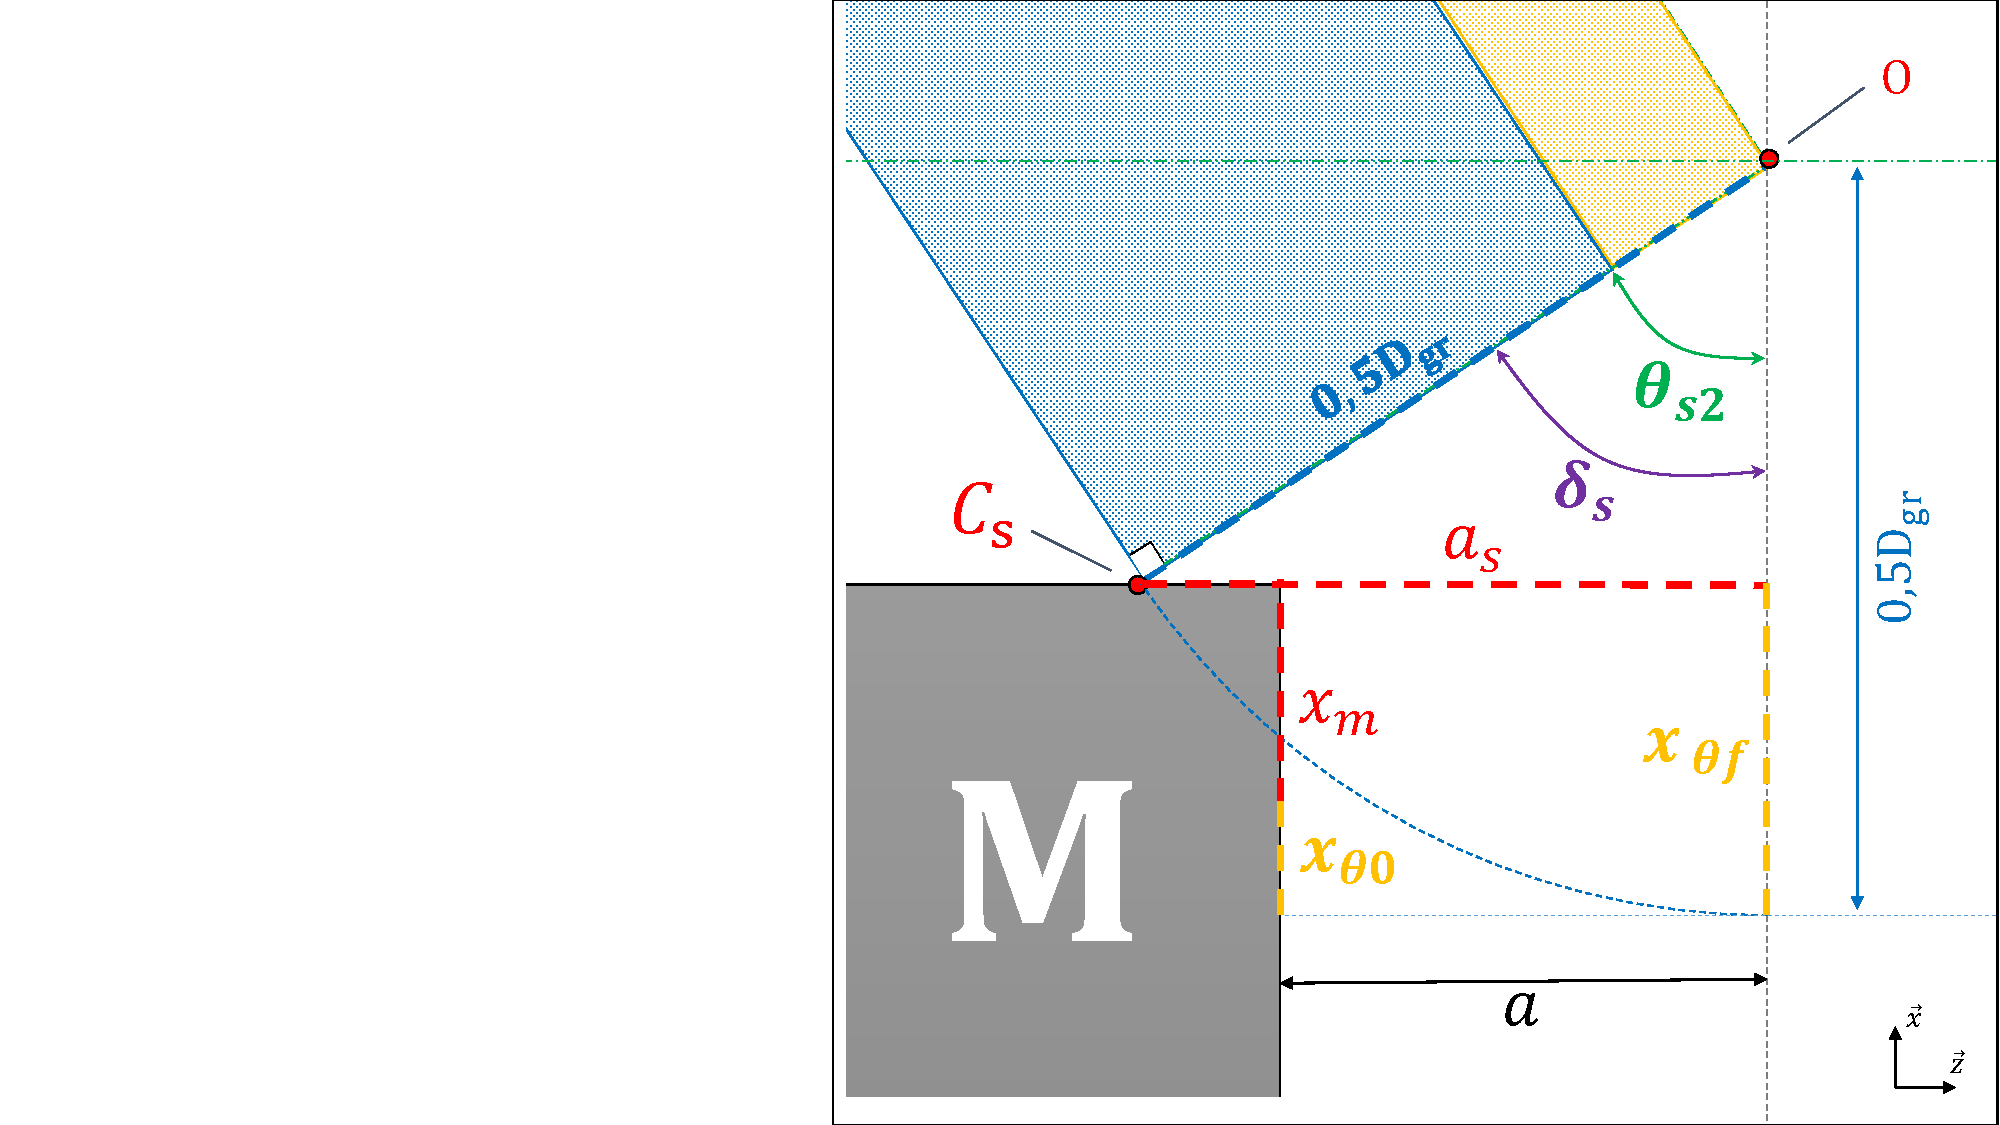
\includegraphics[trim={6cm 0cm 0cm 0cm},clip, 					                 width=\textwidth]{../Chap6/Figure/cinematique_pliage_VH_lacher_calculs_saut.pdf}
%	\caption{Schéma de la configuration de pliage de la VH tenant compte de la gaine rigide après le saut}
%	\label{fig:presentation_BDT}
%\end{center}	
%\end{figure} 
%\FloatBarrier   
%%%%%%%%%%%%%%%%%%%%%%%%%%%%%%%%%%%%%
%
%%%%%%%%%%%%%%%%%%%%%%%%%%%%%%%%%
%%%%%%%%%%%%%%%%%%%%%%%%%%%%%%%%%
% \begin{subnumcases}{}
%$$
%a_2 = \dfrac{D_g}{2}\ sin(\theta)
%$$
%\label{eq:An2_a_saut}\\
%$$
%x_{tf} = \sqrt{(a_0-m_0)^2 + {f_0}^2}
%$$
%\label{eq:An2_xtf_saut}\\
%$$
%x_m = x_{tf} - x_{t0}
%$$
%\label{eq:An2_xm2}
%\end{subnumcases} 
%\label{eq:An2_apres_saut}
%%%%%%%%%%%%%%%%%%%%%%%%%%%%%%%%%
